\documentclass{article}
\usepackage[italian]{babel}
\usepackage[utf8]{inputenc}
\usepackage{fancyhdr}
\usepackage{tikz}
\usepackage{amsmath}
\usepackage{amssymb}
\usepackage{amsthm}
\usepackage{amsfonts}
\usepackage{color}
\usepackage{circuitikz}
\usepackage[margin=2cm]{geometry}
\usepackage[scientific-notation=true]{siunitx}
\usepackage{titlesec}
\usepackage{graphics}

\titleformat{\paragraph}
  {\normalfont\normalsize\bfseries}{\theparagraph}{1em}{}
\titlespacing*{\paragraph}
  {0pt}{3.25ex plus 1ex minus .2ex}{1.5ex plus .2ex}

\title{Misura della caratteristica di un transistor BJT P-N-P in configurazione a emettitore comune}
\date{Quarto turno}
\author{Bertasi Leonardo, Perniola Davide }
\begin{document}
\maketitle
\section{Introduzione} 
Il transistor BJT è un dispositivo bipolare a tre terminali, costituito quindi da tre regioni di semiconduttore con drogaggio alternato
p-n-p o n-p-n. Le tre regioni sono chiamate emettitore, base e collettore. In questa prova abbiamo utilizzato transistor BJT 2N3906(BU) Silicio P-N-P in configuarzione a emettitore comune
e misurato, utilizzando due diverse correnti di base $I_B$, la caratteristica di uscita, ovvero la corrente di collettore $I_C$ in funzione della tensione tra collettore ed emettitore $V_{CE}$.
Inoltre durante la prova sono stati utilizzati due potenziometri da $100k\Omega$ e $1k\Omega$, un alimentatore di bassa tensione un multimetro digitale e un oscilloscopio.
Il circuito realizzato è riporato in Figura 1.



\begin{figure}[]
  \centering
  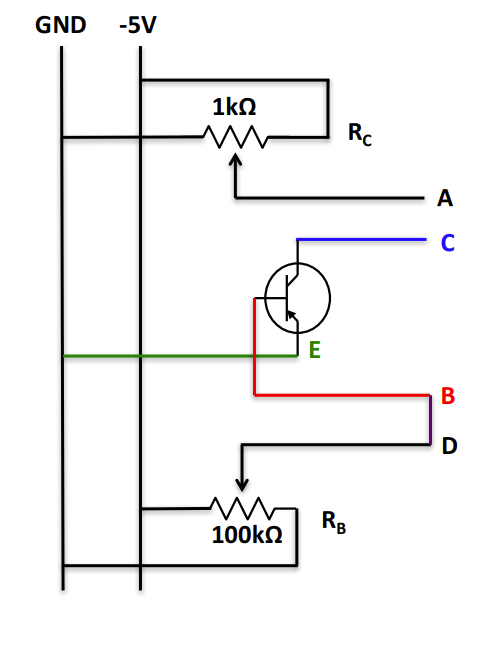
\includegraphics[scale=0.55]{Transis.png}
  \qquad
  \caption{\textit{Rappresentazione schematica del circuito realizzato. }}
\end{figure}



\section{Risultati}
In Tabella 1 e 2 sono riporate le misure dei valori di $I_C$ e $V_{CE}$ effettuate con corrente di base $I_B$ rispettivamente di $(-0.21\pm 0.02) mA$ e $(-0.11\pm 0.02)mA$.
Gli errori sui valori misurati con l'oscilloscopio sono stati ricavati considerando la somma quadratica dell'errore sulla lettura, sullo zero e del costruttore, secondo la relazione\\
\\
$\sigma = \sqrt{(\sigma_L+\sigma_Z)^2+\sigma_C^2} $\\



\begin{table}[]
  \centering
 \mbox{%
\begin{tabular}{|c|c|c|}

\hline
$F.S(mV/div)$ & $V(mV)$ & $I(mA)$\\
\hline

$1000$ & $-4000\pm{156}$ & $-37.54\pm{0.57}$ \\
$1000$ & $-3800\pm{152}$ & $-36.69\pm{0.56}$ \\
$1000$ & $-3600\pm{147}$ & $-36.41\pm{0.56}$ \\
$500$ & $-3400\pm{114}$ & $-35.83\pm{0.55}$ \\
$500$ & $-3200\pm{108}$ & $-35.65\pm{0.54}$ \\
$500$ & $-3000\pm{103}$ & $-35.53\pm{0.54}$ \\
$500$ & $-2800\pm{98}$ & $-35.16\pm{0.54}$ \\
$500$ & $-2600\pm{93}$ & $-34.78\pm{0.53}$ \\
$500$ & $-2400\pm{88}$ & $-34.53\pm{0.53}$ \\
$500$ & $-2200\pm{83}$ & $-34.10\pm{0.52}$ \\
$500$ & $-2000\pm{78}$ & $-33.85\pm{0.52}$ \\
$500$ & $-1800\pm{74}$ & $-33.37\pm{0.51}$ \\
$500$ & $-1600\pm{69}$ & $-32.82\pm{0.50}$ \\
$500$ & $-1400\pm{65}$ & $-32.62\pm{0.50}$ \\
$500$ & $-1200\pm{62}$ & $-32.08\pm{0.49}$ \\
$500$ & $-1000\pm{58}$ & $-31.54\pm{0.48}$ \\
$500$ & $-900\pm{57}$ & $-31.18\pm{0.48}$ \\
$500$ & $-800\pm{55}$ & $-30.79\pm{0.47}$ \\
$500$ & $-700\pm{54}$ & $-30.22\pm{0.46}$ \\
$500$ & $-600\pm{53}$ & $-29.46\pm{0.45}$ \\
$200$ & $-500\pm{25}$ & $-28.67\pm{0.44}$ \\
$100$ & $-450\pm{17}$ & $-27.51\pm{0.42}$ \\
$100$ & $-400\pm{16}$ & $-26.78\pm{0.41}$ \\
$100$ & $-350\pm{15}$ & $-25.82\pm{0.40}$ \\
$100$ & $-300\pm{13}$ & $-24.60\pm{0.48}$ \\
$100$ & $-250\pm{13}$ & $-22.93\pm{0.45}$ \\
$100$ & $-200\pm{12}$ & $-20.75\pm{0.32}$ \\
$100$ & $-150\pm{11}$ & $-15.03\pm{0.24}$ \\
$100$ & $-100\pm{10}$ & $-9.24\pm{0.15}$ \\
$50$ & $-80\pm{6}$ & $-4.48\pm{0.08}$ \\
$50$ & $-60\pm{5}$ & $-2.31\pm{0.04}$ \\
$50$ & $-50\pm{5}$ & $-1.43\pm{0.03}$ \\

\hline
\end{tabular}
 }
 \caption{\textit{Risultati delle misure effettuate con corrente di base $I_B=-210\mu A$}}
\end{table}




\begin{table}[]
  \centering
 \mbox{%
\begin{tabular}{|c|c|c|}

\hline
$F.S(mV/div)$ & $V(mV)$ & $I(mA)$\\
\hline

$1000$ & $-4000\pm{156}$ & $-19.32\pm{0.30}$ \\
$1000$ & $-3800\pm{152}$ & $-19.37\pm{0.30}$ \\
$1000$ & $-3600\pm{147}$ & $-19.28\pm{0.30}$ \\
$500$ & $-3400\pm{114}$ & $-19.15\pm{0.30}$ \\
$500$ & $-3200\pm{108}$ & $-19.15\pm{0.30}$ \\
$500$ & $-3000\pm{103}$ & $-19.03\pm{0.30}$ \\
$500$ & $-2800\pm{98}$ & $-18.96\pm{0.29}$ \\
$500$ & $-2600\pm{93}$ & $-18.62\pm{0.29}$ \\
$500$ & $-2400\pm{88}$ & $-18.55\pm{0.29}$ \\
$500$ & $-2200\pm{83}$ & $-18.40\pm{0.29}$ \\
$500$ & $-2000\pm{78}$ & $-18.29\pm{0.28}$ \\
$500$ & $-1800\pm{74}$ & $-17.92\pm{0.28}$ \\
$500$ & $-1600\pm{69}$ & $-17.70\pm{0.28}$ \\
$500$ & $-1400\pm{65}$ & $-17.53\pm{0.27}$ \\
$500$ & $-1200\pm{62}$ & $-17.34\pm{0.27}$ \\
$500$ & $-1000\pm{58}$ & $-17.25\pm{0.27}$ \\
$500$ & $-900\pm{57}$ & $-17.03\pm{0.27}$ \\
$500$ & $-800\pm{55}$ & $-16.91\pm{0.26}$ \\
$500$ & $-700\pm{54}$ & $-16.83\pm{0.26}$ \\
$500$ & $-600\pm{53}$ & $-16.57\pm{0.26}$ \\
$200$ & $-500\pm{25}$ & $-16.58\pm{0.26}$ \\
$100$ & $-450\pm{17}$ & $-16.40\pm{0.26}$ \\
$100$ & $-400\pm{16}$ & $-16.27\pm{0.25}$ \\
$100$ & $-350\pm{15}$ & $-16.08\pm{0.25}$ \\
$100$ & $-300\pm{13}$ & $-15.57\pm{0.24}$ \\
$100$ & $-250\pm{13}$ & $-14.79\pm{0.23}$ \\
$100$ & $-200\pm{12}$ & $-13.94\pm{0.22}$ \\
$100$ & $-150\pm{11}$ & $-11.25\pm{0.18}$ \\
$100$ & $-100\pm{10}$ & $-6.13\pm{0.10}$ \\
$50$ & $-80\pm{6}$ & $-2.87\pm{0.05}$ \\
$50$ & $-60\pm{5}$ & $-1.31\pm{0.03}$ \\
$50$ & $-50\pm{5}$ & $-0.83\pm{0.02}$ \\

\hline
\end{tabular}
 }
 \caption{\textit{Risultati delle misure effettuate con corrente di base $I_B=-110\mu A$}}
\end{table}

In Figura 2 sono riportati i risultati del fit ai dati sperimentali, effettuato nella regione attiva ($|V_{CE}|>1$). Per ciascun valore di $V_B$, il parametro
$p_0$ rappresenta la tensione di early, $p_1$

\begin{figure}[]
  \centering
  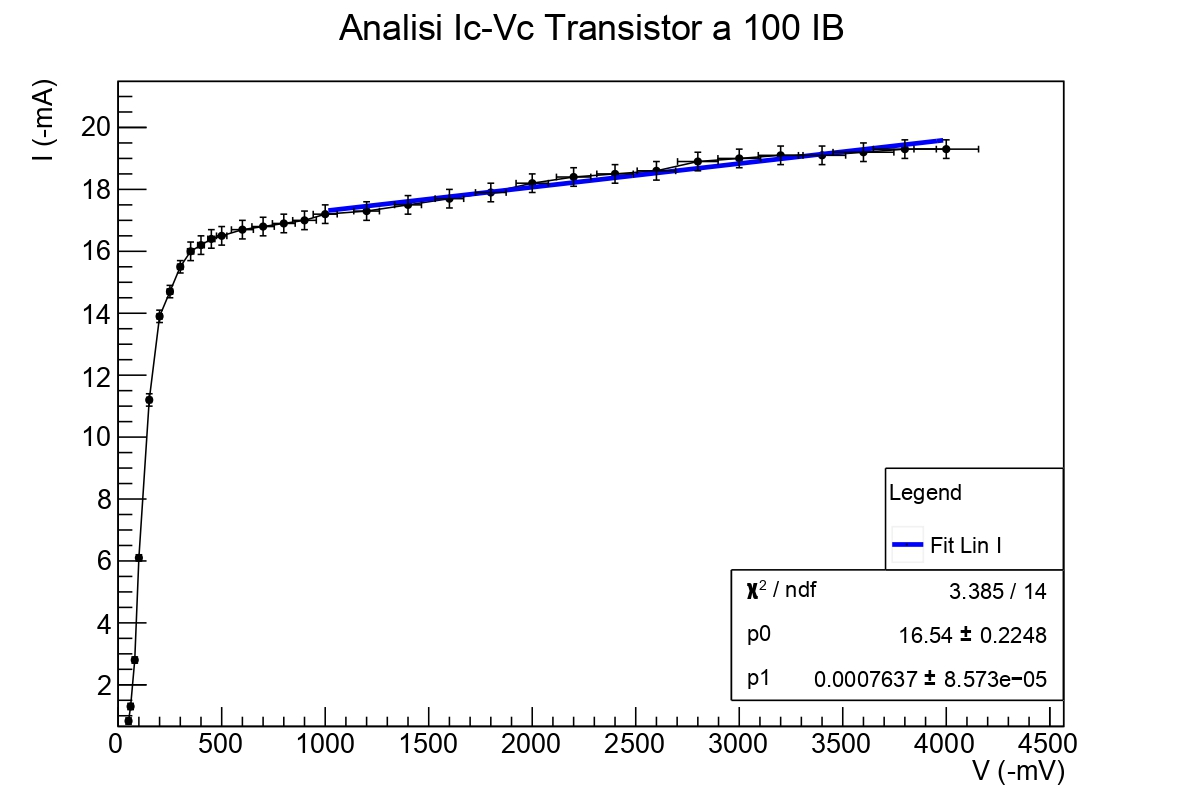
\includegraphics[scale=0.55]{Trans100.jpg}
  \qquad
  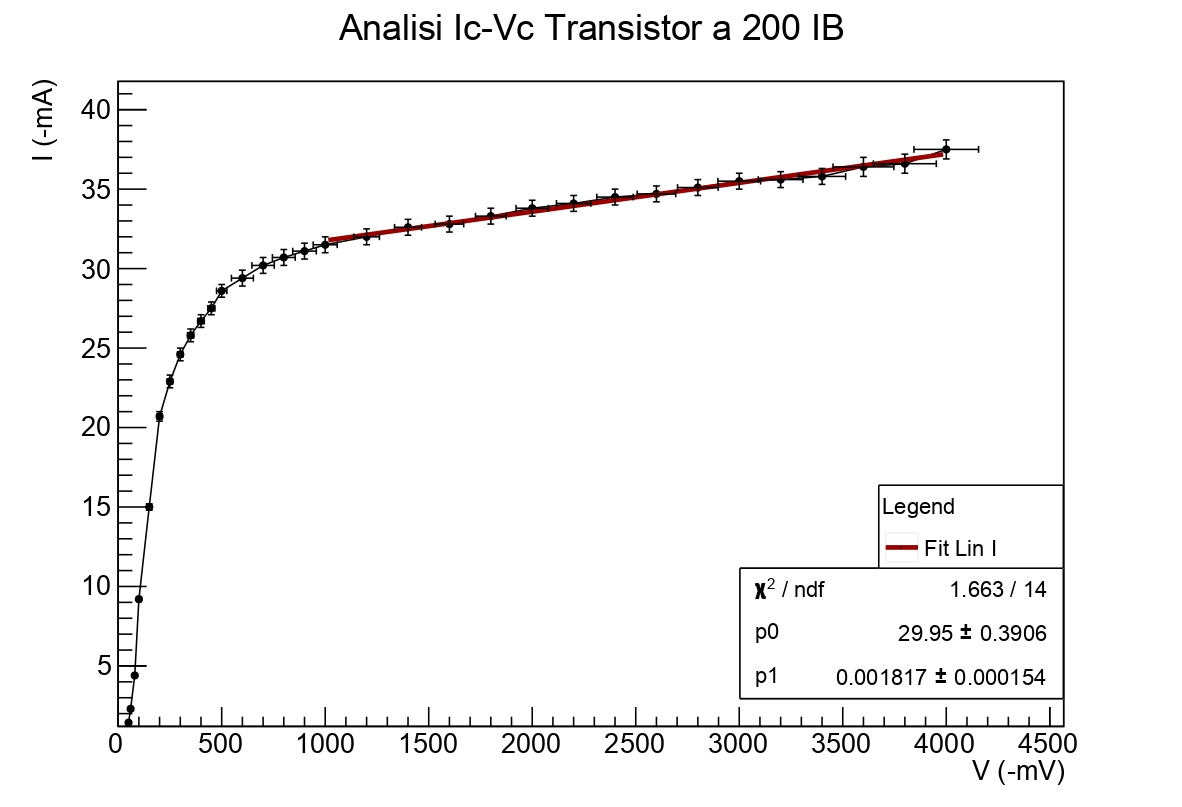
\includegraphics[scale=0.55]{Trans200.jpg}
  \qquad
  \caption{\textit{Rappresentazione schematica del circuito realizzato. }}
\end{figure}



\section{Conclusioni}


Lo scopo di questa prova è stato misurare le caratterisrticge e 
Lo scopo di questa prova è stato misurare le caratterisrticge e 
Lo scopo di questa prova è stato misurare le caratterisrticge e 
Lo scopo di questa prova è stato misurare le caratterisrticge e 









\end{document}
